\documentclass[tikz,border=10pt]{standalone}

\usepackage{amsmath, amssymb, bm}
\usepackage{tikz}
\usetikzlibrary{positioning, arrows.meta, shapes.geometric, calc, fit, backgrounds}

\newcommand{\R}{\mathbb{R}}

\begin{document}

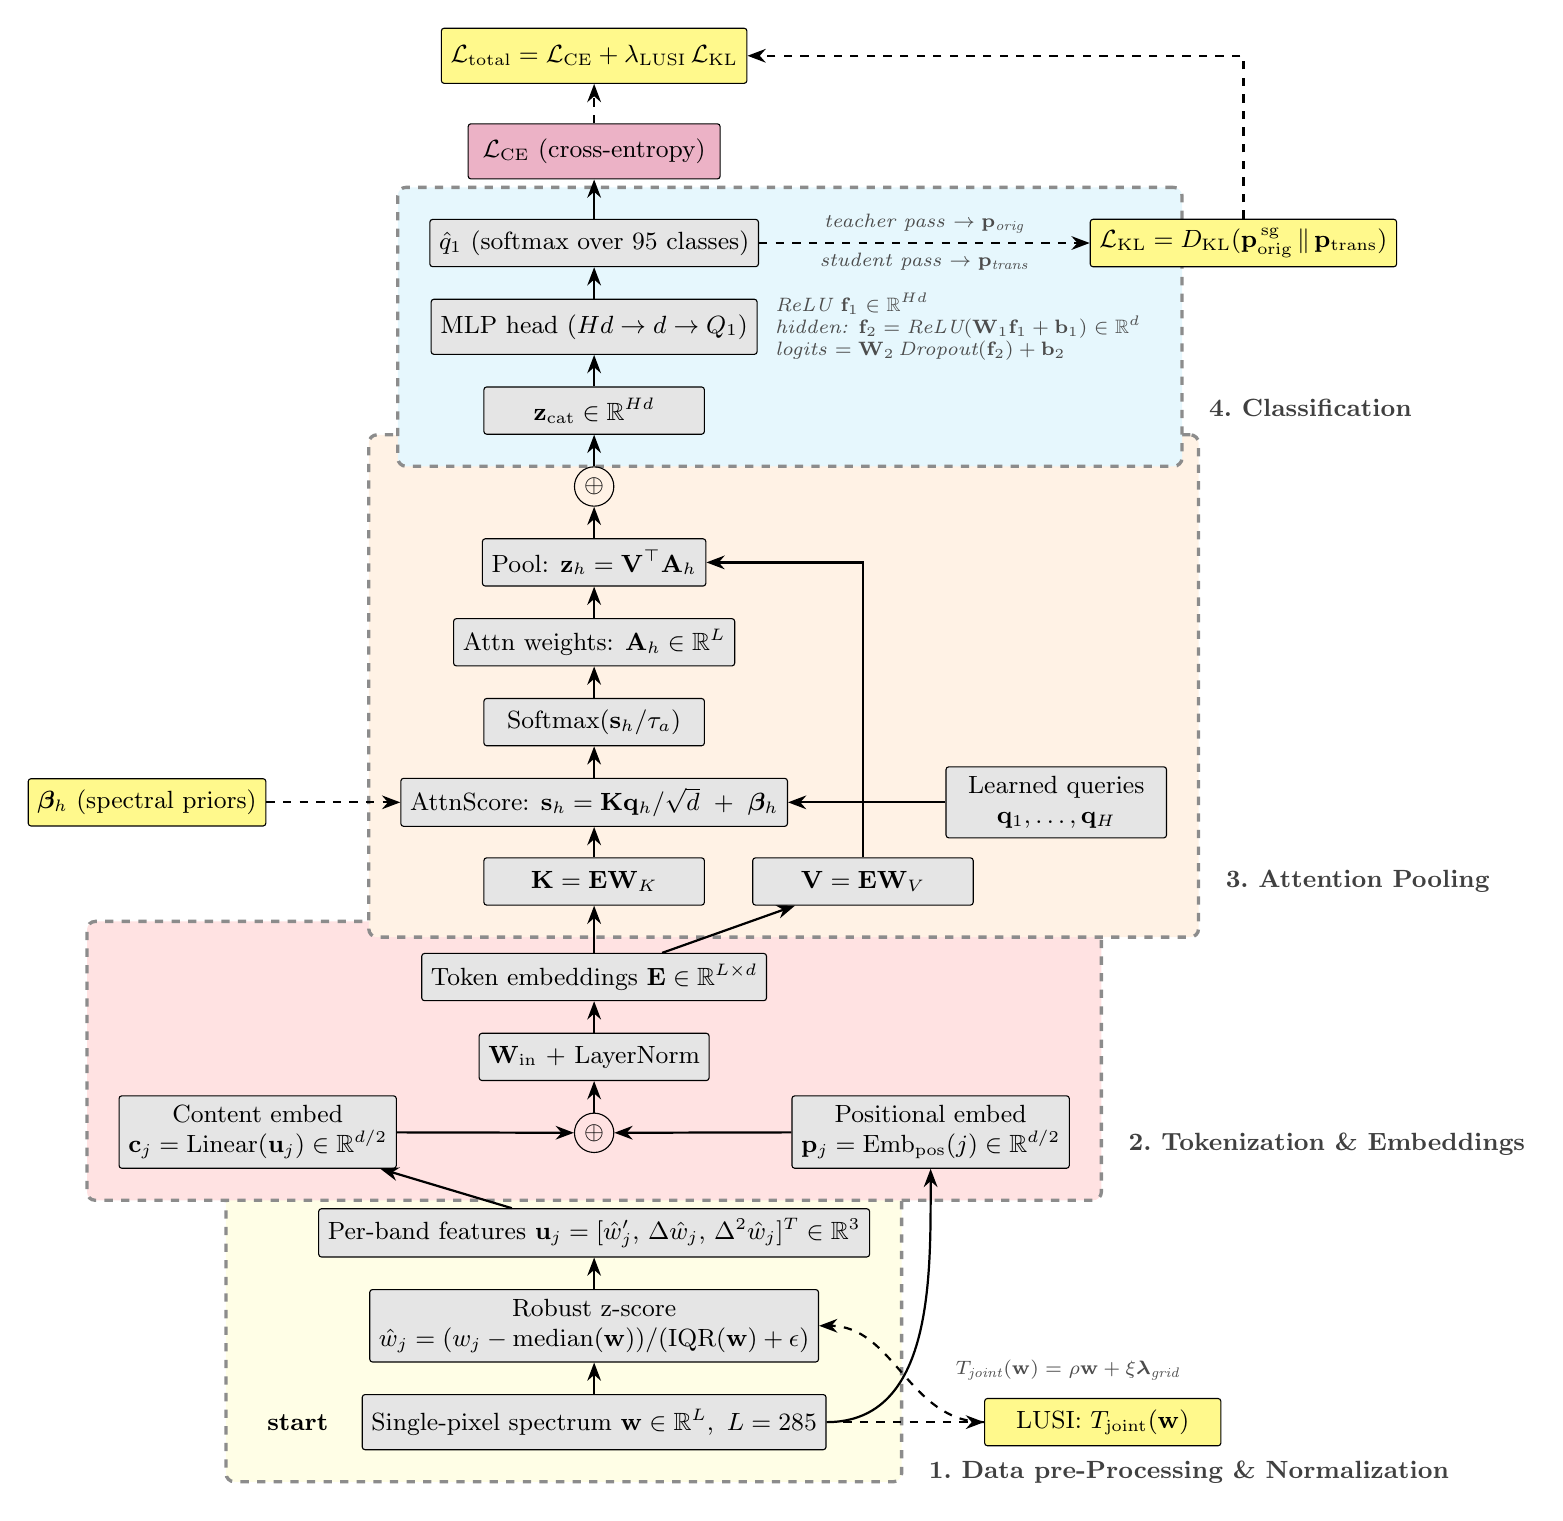
\begin{tikzpicture}[
  font=\small,
  node distance=4mm,
  >=Stealth,
  % "Attention is all you need"-style color palette:
  block/.style   ={draw, fill=gray!20, rounded corners=1pt, minimum width=32mm, minimum height=7mm, align=center},
  embed/.style   ={draw, fill=gray!20,   rounded corners=1pt, minimum width=28mm, minimum height=6mm, align=center}, % embeddings
  attn/.style    ={draw, fill=gray!20,   rounded corners=1pt, minimum width=28mm, minimum height=6mm, align=center}, % attention
  ff/.style      ={draw, fill=gray!20,   rounded corners=1pt, minimum width=32mm, minimum height=7mm, align=center}, % feed-forward
  linear/.style  ={draw, fill=gray!20,   rounded corners=1pt, minimum width=28mm, minimum height=6mm, align=center}, % linear layers
  softmax/.style ={draw, fill=gray!20,   rounded corners=1pt, minimum width=28mm, minimum height=6mm, align=center}, % softmax
  tensor/.style  ={draw, fill=gray!20,   rounded corners=1pt, minimum width=28mm, minimum height=6mm, align=center}, % data-flow tensors
  queryv/.style  ={draw, fill=gray!20,   rounded corners=1pt, minimum width=28mm, minimum height=6mm, align=center}, % learned queries (attention input)
  bias/.style    ={draw, fill=yellow!45, rounded corners=1pt, minimum width=28mm, minimum height=6mm, align=center}, % physics prior (optional)
  lusi/.style    ={draw, fill=yellow!45, rounded corners=1pt, minimum width=30mm, minimum height=6mm, align=center}, % LUSI branch (optional)
  loss/.style    ={draw, fill=purple!30,   rounded corners=1pt, minimum width=32mm, minimum height=7mm, align=center}, % loss boxes
  op/.style      ={draw, circle, minimum size=5mm, inner sep=0pt},
  arrow/.style   ={-Stealth, thick},
  group/.style   ={draw=gray!90, very thick, dashed, rounded corners=3pt, inner sep=4mm, fill=blue!3},
  grouptitle/.style ={font=\small\bfseries, text=gray!50!black, anchor=north west},
]

% --- Input & preprocessing ---
\node[block]                        (spec) {Single-pixel spectrum $\mathbf{w} \in \R^{L},\ L=285$};
\node[font=\small\bfseries, left=3mm of spec] (startlabel) {start};
\node[block, above=of spec]         (norm) {Robust z-score\\ $\hat{w}_j = (w_j - \text{median}(\mathbf{w}))/(\text{IQR}(\mathbf{w}) + \epsilon)$};
\node[tensor, above=of norm]        (uj)   {Per-band features $\mathbf{u}_j = [\hat{w}'_j,\, \Delta\hat{w}_j,\, \Delta^2\hat{w}_j]^T \in \R^3$};

% --- Split embedding (content + position) ---
\node[embed, above left =5mm and -10mm of uj] (cj) {Content embed\\ $\mathbf{c}_j = \text{Linear}(\mathbf{u}_j) \in \R^{d/2}$};
\node[embed, above right=5mm and -10mm of uj] (pj) {Positional embed\\ $\mathbf{p}_j = \text{Emb}_{\text{pos}}(j) \in \R^{d/2}$};
\node[op,    above=7mm of uj]       (cat1) {$\oplus$};
\node[linear, above=of cat1]        (Win)  {$\mathbf{W}_{\text{in}}$ $+$ LayerNorm};
\node[embed, above=of Win]          (E)    {Token embeddings $\mathbf{E} \in \R^{L \times d}$};

% --- K, V projections + separate learned queries ---
\node[linear, above =6mm and 8mm of E] (K) {$\mathbf{K} = \mathbf{E}\mathbf{W}_K$};
\node[linear, right=6mm of K] (V) {$\mathbf{V} = \mathbf{E}\mathbf{W}_V$};

% --- Cross-attention pipeline ---
\node[attn, above=16mm of E]        (score) {AttnScore: $\mathbf{s}_h = \mathbf{K}\mathbf{q}_h/\sqrt{d}\ +\ \bm{\beta}_h$};
\node[queryv, right=20mm of score]      (q) {Learned queries\\ $\mathbf{q}_1,\ldots,\mathbf{q}_H$};
\node[bias,  left=17mm of score]    (beta)  {$\bm{\beta}_h$ (spectral priors)};

\node[softmax, above=of score]      (sm)    {Softmax($\mathbf{s}_h / \tau_a$)};
\node[attn, above=of sm]            (A)     {Attn weights: $\mathbf{A}_h \in \R^L$};
\node[attn, above=of A]             (pool)  {Pool: $\mathbf{z}_h = \mathbf{V}^\top \mathbf{A}_h$};

% --- Head concat + classifier ---
\node[op,    above=of pool]         (cat2) {$\oplus$};
\node[tensor, above=of cat2]        (zcat) {$\mathbf{z}_{\text{cat}} \in \R^{Hd}$};
\node[ff,    above=of zcat]         (mlp)  {MLP head ($Hd \to d \to Q_1$)};
\node[font=\scriptsize\itshape, text=gray!60!black, align=left, right=1mm of mlp]
      (mlpdetail)
      {ReLU $\mathbf{f}_1 \in \R^{Hd}$\\
       hidden: $\mathbf{f}_2 = \text{ReLU}(\mathbf{W}_1 \mathbf{f}_1 + \mathbf{b}_1) \in \R^{d}$\\
       logits $= \mathbf{W}_2\,\text{Dropout}(\mathbf{f}_2) + \mathbf{b}_2$};
\node[softmax, above=of mlp]         (out) {$\hat{q}_{1}$ (softmax over 95 classes)};

% --- Losses ---
\node[loss, above=5mm of out]            (ce)   {$\mathcal{L}_{\text{CE}}$ (cross-entropy)};
\node[loss, fill=yellow!45, above=5mm of ce]  (total){$\mathcal{L}_{\text{total}} = \mathcal{L}_{\text{CE}} + \lambda_{\text{LUSI}}\,\mathcal{L}_{\text{KL}}$};

% --- LUSI branch (optional, dashed) ---
\node[lusi,  right=10mm and 20mmof spec]    (T)    {LUSI: $T_{\text{joint}}(\mathbf{w})$};
\node[font=\scriptsize\itshape, text=gray!60!black, align=left, anchor=south west]
      at ($(T.north east) + (-35mm, 1mm)$)
      (Tdetail)
      {$T_{\text{joint}}(\mathbf{w}) = \rho \mathbf{w} + \xi \bm{\lambda}_{\text{grid}}$};
\node[lusi,  right=42mm of out]     (kl)   {$\mathcal{L}_{\text{KL}} = D_{\text{KL}}(\mathbf{p}_{\text{orig}}^{\,\mathrm{sg}} \,\|\, \mathbf{p}_{\text{trans}})$};

% --- Main arrows ---
\draw[arrow] (spec) -- (norm);   \draw[arrow] (norm) -- (uj);
\draw[arrow] (uj)   -- (cj);
\draw[arrow] (spec.east) to[out=0, in=-90] (pj.south);
\draw[arrow] (cj)   -- (cat1);   \draw[arrow] (pj)   -- (cat1);
\draw[arrow] (cat1) -- (Win);    \draw[arrow] (Win)  -- (E);
\draw[arrow] (E)    -- (K);      \draw[arrow] (E)    -- (V);
\draw[arrow] (K)    -- (score);  \draw[arrow] (q)    -- (score);
\draw[arrow, dashed] (beta) -- (score);
\draw[arrow] (score)-- (sm);     \draw[arrow] (sm)   -- (A);
\draw[arrow] (A)    -- (pool);   \draw[arrow] (V)    |- (pool);
\draw[arrow] (pool) -- (cat2);   \draw[arrow] (cat2) -- (zcat);
\draw[arrow] (zcat) -- (mlp);    \draw[arrow] (mlp)  -- (out);

% --- Loss arrows ---
\draw[arrow] (out) -- (ce);
\draw[arrow, dashed] (ce)  -- (total);

% --- LUSI arrows (dashed) ---
\draw[arrow, dashed] (spec) -- (T);
\draw[arrow, dashed] (T) to[out=180, in=0] (norm.east);  % student pass: transformed spectrum re-enters pipeline at norm
\draw[arrow, dashed] (out) -- node[above, font=\scriptsize\itshape, text=gray!60!black] {teacher pass $\to \mathbf{p}_{\text{orig}}$} node[below, font=\scriptsize\itshape, text=gray!60!black] {student pass $\to \mathbf{p}_{\text{trans}}$} (kl);
\draw[arrow, dashed] (kl.north) |- (total.east);

% --- Group boxes (drawn on background so they sit behind the nodes) ---
%   Coloring follows "Attention is all you need" (Vaswani et al., 2017):
%     embeddings -> pink, multi-head attention -> orange, feed-forward -> cyan.
%     Pre-processing has no Vaswani analog; a neutral light tan is used.
\begin{scope}[on background layer]
  \node[group, fill=yellow!10,  fit=(spec)(norm)(uj)(startlabel)] (g1) {};
  \node[group, fill=pink!45,   fit=(cj)(pj)(cat1)(Win)(E)] (g2) {};
  \node[group, fill=orange!10, fit=(K)(V)(q)(score)(sm)(A)(pool)(cat2)] (g3) {};
  \node[group, fill=cyan!10,   fit=(zcat)(mlp)(mlpdetail)(out)] (g4) {};
\end{scope}
\node[grouptitle] at ([xshift=2mm,yshift=4mm]g1.south east) {1.\ Data pre-Processing \& Normalization};
\node[grouptitle] at ([xshift=2mm,yshift=10mm]g2.south east) {2.\ Tokenization \& Embeddings};
\node[grouptitle] at ([xshift=2mm,yshift=10mm]g3.south east) {3.\ Attention Pooling};
\node[grouptitle] at ([xshift=2mm,yshift=10mm]g4.south east) {4.\ Classification};

\end{tikzpicture}

\end{document}
